%% Based on a TeXnicCenter-Template by Tino Weinkauf.
%%%%%%%%%%%%%%%%%%%%%%%%%%%%%%%%%%%%%%%%%%%%%%%%%%%%%%%%%%%%%

%%%%%%%%%%%%%%%%%%%%%%%%%%%%%%%%%%%%%%%%%%%%%%%%%%%%%%%%%%%%%
%% Preamble
%%%%%%%%%%%%%%%%%%%%%%%%%%%%%%%%%%%%%%%%%%%%%%%%%%%%%%%%%%%%%
\documentclass[onecolumn, letterpaper, 12pt]{article}
\usepackage{times,color,amsfonts,amsmath,amssymb,amsthm,comment,graphicx,cite}
%\documentclass[letterpaper,oneside,11pt]{letter}
% Alternative Options:
%	Paper Size: a4paper / a5paper / b5paper / letterpaper / legalpaper / executivepaper
% Duplex: oneside / twoside
% Base Font Size: 10pt / 11pt / 12pt


%% Language %%%%%%%%%%%%%%%%%%%%%%%%%%%%%%%%%%%%%%%%%%%%%%%%%
%%%%%%%%%\usepackage[USenglish]{babel} %francais, polish, spanish, ... NOTE:  Requires you find and download a dictionary file.  Don't use this unless you run into problems.
%%%%%%%%%\usepackage[T1]{fontenc}
%%%%%%%%%\usepackage[ansinew]{inputenc}

\usepackage{algorithm}
\usepackage{algpseudocode}
\usepackage{float}
\usepackage{graphicx}


%% Math Packages %%%%%%%%%%%%%%%%%%%%%%%%%%%%%%%%%%%%%%%%%%%%
%\usepackage{amsmath}
%\usepackage{amsthm}
%\usepackage{amsfonts}
%\usepackage{amssymb}
%\usepackage{array,MnSymbol}


%% Line Spacing %%%%%%%%%%%%%%%%%%%%%%%%%%%%%%%%%%%%%%%%%%%%%
\usepackage{setspace}
\singlespacing        %% 1-spacing (default)
%\onehalfspacing       %% 1,5-spacing
%\doublespacing        %% 2-spacing, this is nice for drafts and required sometimes for blind paper submit.


%% Other Packages %%%%%%%%%%%%%%%%%%%%%%%%%%%%%%%%%%%%%%%%%%%
\usepackage{fancyhdr} %%Fancy headings
\pagestyle{fancy} %You would not do this for a publication unless asked
\fancyhead[L]{Danielle Sarafian}
\fancyhead[C]{} %stuff to be centered at the top of the page
\fancyhead[R]{0/1 Knapsack, page \thepage}
\fancyfoot[L]{} %stuff for left margin at the bottom of the page
\fancyfoot[C]{} %stuff to be centered at the bottom of the page
\fancyfoot[R]{} %stuff to be right-justified against the right margin at the bottom of the page


\usepackage{listings} %Preserves formatting of java, C++, or other code



%%%%%%
%%%%%% Theorem like environments for proofs
%%%%%%
%%%%%\newtheorem{problem}{Problem}%
%%%%%%\numberwithin{problem}{section}
%%%%%\newtheorem{theorem}{Theorem}%
%%%%%\newtheorem{acknowledgment}{Acknowledgment}%
%%%%%%\newtheorem{algorithm}{Algorithm}%
%%%%%\newtheorem{assumption}{Assumption}%
%%%%%\newtheorem{axiom}{Axiom}%
%%%%%\newtheorem{case}{Case}%
%%%%%\numberwithin{case}{problem}
%%%%%\newtheorem{claim}{Claim}%
%%%%%\newtheorem{conclusion}{Conclusion}
%%%%%\newtheorem{condition}{Condition}
%%%%%\numberwithin{condition}{problem}
%%%%%\numberwithin{condition}{subsection}
%%%%%\newtheorem{conjecture}{Conjecture}
%%%%%\newtheorem{corollary}{Corollary}
%%%%%\newtheorem{criterion}{Criterion}
%%%%%\newtheorem{definition}{Definition}
%%%%%\numberwithin{definition}{section}
%%%%%\newtheorem{example}{Example}
%%%%%\newtheorem{exercise}{Exercise}%
%%%%%\newtheorem{lemma}{Lemma}%
%%%%%\newtheorem{notation}{Notation}%
%%%%%\theoremstyle{remark}
%%%%%\newtheorem{question}{Question}%
%%%%%\numberwithin{question}{problem}
%%%%%\theoremstyle{plain}
%%%%%\newtheorem{answer}{Answer}%
%%%%%\numberwithin{answer}{problem}
%%%%%\newtheorem{proposition}{Proposition}%
%%%%%\newtheorem{remark}{Remark}%
%%%%%\newtheorem{solution}{Solution}%
%%%%%\numberwithin{solution}{section}
%%%%%\newtheorem{summary}{Summary}%
%%%%%\numberwithin{equation}{section}%
%%%%%\newtheorem{option}{Option}
%%%%%




%%%%%%%%%%%%%%%%%%%%%%%%%%%%%%%%%%%%%%%%%%%%%%%%%%%%%%%%%%%%%
%% DOCUMENT
%%%%%%%%%%%%%%%%%%%%%%%%%%%%%%%%%%%%%%%%%%%%%%%%%%%%%%%%%%%%%
\begin{document}

\thispagestyle{empty} %No headings/footers for the first pages.


%% Title Page %%%%%%%%%%%%%%%%%%%%%%%%%%%%%%%%%%%%%%%%%%%%%%%


\title{0/1 Knapsack}
\author{Danielle Sarafian}
\date{16 March 2018}
\maketitle 




\begin{abstract}

This project focuses on and analyzes the strategies used to complete the 0/1 Knapsack problem including sorting by price density and taking the largest density first, sorting by price and taking the largest price first, using the brute force solution, and using the dynamic programming solution.

\end{abstract}
\section{Motivation}
The problem of finding the optimal solution is very important because the optimal solution is the best possible answer. Clearly, having the best answer can be useful in many cases. In some situations, it is important to consider the tradeoff between the optimal solution and the time it takes to find that optimal solution. If finding the optimal solution takes longer than finding a solution that is close to the optimal solution, is it worth it to spend the time finding the optimal solution?

\section{Background}
The 0/1 knapsack problem, as defined by Cormen in \textit{Introduction to Algorithms} is as follows: ``A thief robbing a store finds \textit{n} items. The \textit{i}th item is worth $v_i$ dollars and weighs $w_i$ pounds, where $v_i$ and $w_i$ are integers. The thief wants to take as valuable a load as possible, but he can carry at most \textit{W} pounds in his knapsack, for some integer \textit{W}. Which items should he take?"~\cite{cormen2001introduction}. This analysis could be applied to a real-world scenario when considering items to save during a fire or, like Cormen described, when a thief is taking as valueable a load as possible. Of course, in these situations, the highest price may be a lower priority than the time available, so, an analysis of different methods of taking these items is in order.

The goal of this project is to understand the pros and cons of different solutions to the 0/1 Knapsack problem. I predict that the price density solution will be the fastest and the brute force solution will take the longest time. In addition, I predict that the brute force will always find the optimal solution, but  the other solutions will not always find it, though they may some of the time.


\section{Procedure}
A computer program was written in order to test this problem. This program consisted of different classes for each possible solution: brute force, greedy 1 (taking the item with the largest price first), greedy 2 (using price density), and the dynamic programming solution. For all solutions, the precondition exists that the weights of the items are not larger than the capacity. This is accounted for in the Knapsack class in which random weights and prices are generated. If the random weight exceeds the capacity, the number is regenerated. A class called Item was created in order to represent an item that has a weight and a price. When performing the two greedy solutions, the items needed to be sorted. Heap sort was used to sort these items because its time is $O(nlgn)$ and is the fastest sort, as proven in Project 1. The algorithms for the solutions are below.

\begin{algorithm}[H]
\caption {\textsc{greedyDensity}()}
\label{greedyDensityps}
\begin{algorithmic}[1]
\Procedure{greedyDensity}{}

\Comment{All variables are instance variables initialized in the constructor for this class.}
\For {$i=0$ to $items.length$}
\Comment {items is an array containing objects of type Item}
\State {$temp = items[i].getPriceDensity()$}
\State {$priceDensity[i] = temp$}
\EndFor
\State {finalKnapsack is a new array of size items.length}
\State {$priceDensity = sort.reverseHeapSort(priceDensity)$}
\For {$index = 0$ to $priceDensity.length$}
\If {$items[index].getWeight() <= capacity$}
\State {$finalKnapsack[index] = 1$}
\State {$c=-items[index].getWeight()$}
\State {$capacityFilled=+items.getWeight()$}
\State {$finalPrice =+ items[index].getPrice()$}
\EndIf
\EndFor

\EndProcedure
\end{algorithmic}
\end{algorithm}

\begin{algorithm}[H]
\caption {\textsc{dynamicProgramming}(profit, weight, c, array)}
\label{dpsolveps}
\begin{algorithmic}[1]
\Procedure{dynamicProgramming}{profit, weight, c, array}

\State {$numObj = profit.length$}
\State {$yMax = min(weight[numObj-1], c)$}
\For {$y=0$ to $yMax$}
\State {$array [numObj][y] = 0$}
\EndFor
\For {$y=weight[numObj$ to $c$}
\State {$array [numObj][y] = profit[numObj]$}
\EndFor
\For {$i=numObj-1$ down to 0}
\State {$yMax = min(weight[i]-1, c)$}
\For {$y = 0$ to $yMax$}
\State {$array[i][y] = array [i+1][y]$}
\EndFor
\For {$y = weight[i]$ to $c$}
\State {$array[i][y] = max(array[i+1][y], array[i+1][y-weight[i]]+profit[i])$}
\EndFor
\EndFor
\State {$array[1][c] = array[2][c]$}
\If {$c >= weight[1]$}
\State {$array[1][c] = max(array[1][c], array[2][c-weight[1]]+profit[1])$}
\EndIf
\State {solution is a new array of length profit.length}
\State{traceback(array, weight, profit, c, solution)}

\Comment{Algorithm from Sahni}
\EndProcedure
\end{algorithmic}
\end{algorithm}

\begin{algorithm}[H]
\caption {\textsc{traceback}(array, weight, price, c, solution)}
\label{tracebackps}
\begin{algorithmic}[1]
\Procedure{traceback}{array, weight, price, c, solution}

\State {$numObj = weight.length-1$}
\For {$i = 0$ to $numObj-1$}
\If {$array[i][c] == array[i+1][c]$}
\State {$solution[i] = 0;$}
\EndIf
\State {else} 
\State {$solution[i] = 1$} 
\State {$c -= weight[i]$}
\State {end else}
\EndFor
\State {$solution[numObj] = (array[numObj][c]>0) ? 1 : 0$}

\Comment{Algorithm from Sahni}
\EndProcedure
\end{algorithmic}
\end{algorithm}

\begin{algorithm}[H]
\caption {\textsc{bruteForce}(num)}
\label{bruteforceps}
\begin{algorithmic}[1]
\Procedure{bruteForce}{num}

\If{$num < 0$}
\State {$weight = 0$}
\State {$price = 0$}
\For {$i = 0$ to $numItems$}
\If {$current[i]$}
\State {$weight = weight + items[i].getWeight()$}
\State {$price = price + items[i].getPrice()$}
\EndIf
\EndFor
\If {$weight <= capacity$ and $price > best$}
\State {$best = price$}
\State {$capacityFilled = weight$}
\State {copySolution()}
\EndIf
\State {return}
\EndIf
\State {$current[num] = true$}
\State {solve(num-1)}
\State {$current[num] = false$}
\State {solve(num-1)}


\Comment{Based on code from GitHub, Inc.}
\EndProcedure
\end{algorithmic}
\end{algorithm}

\begin{algorithm}[H]
\caption {\textsc{greedyPrice}()}
\label{greedyPriceps}
\begin{algorithmic}[1]
\Procedure{greedyPrice}{}

\Comment {PRECONDITION: price array is sorted lowest to highest value}
\For {$i = sortedPrice.length-1$ down to $0$}
\If {(currentC is nonnegative, currentC is less than c, and c-currentC is nonnegative)}
\State {$solution[i] = 1$}
\State {$currentC = currentC - (int)(sortedPrice[i].getWeight())$}
\EndIf
\State {else }
\State{$solution[i] = 0$}
\State {end else}
\EndFor


\EndProcedure
\end{algorithmic}
\end{algorithm}

\section{Testing}
\subsection{Testing Plan and Results}
In order to test this, three trials were run for all of the data and for three of the solutions (price density, dynamic programming, and largest price). Brute force began to take too long after the test with 25 elements. The solution methods were run with capacities of 5, 15, 25, 35, 45, 55, 65, 75 , 85, and 95. The highest price and weight possible were set at 100, though if the random weight generated exceeded the capacity for the knapsack, it would be regenerated. The solutions were tested with an array of 10 random items.

\begin{figure}[H]
\centering
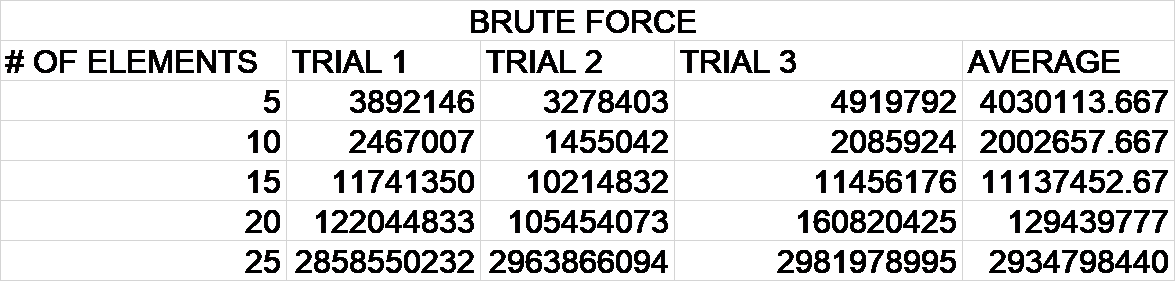
\includegraphics[width=0.8\linewidth]{./bruteForceTable.png}
\caption{Results from Brute Force Solution}
\label{fig:bruteForceResults}
\end{figure}

\begin{figure}[H]
\centering
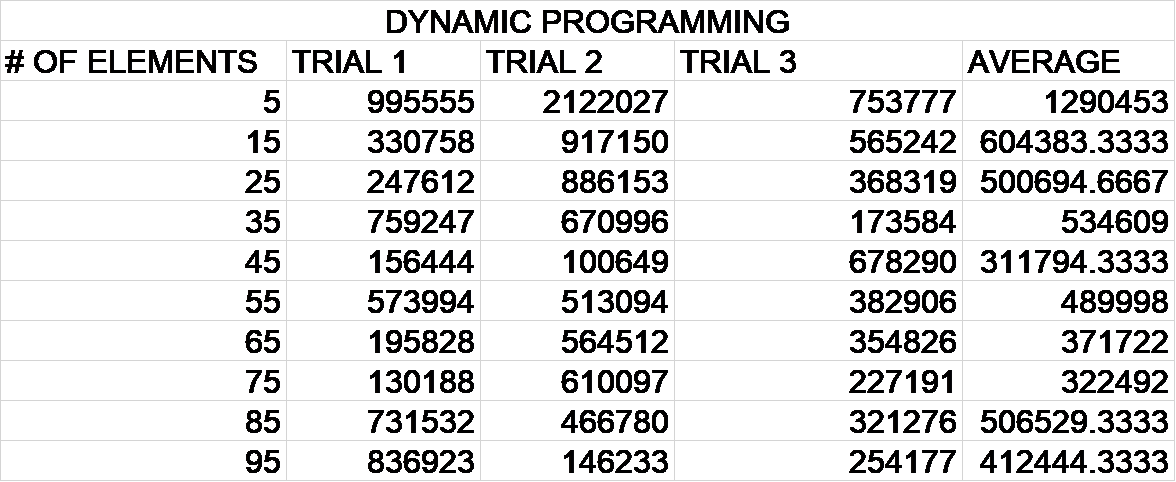
\includegraphics[width=0.8\linewidth]{./dynamicProgrammingTable.png}
\caption{Results from Dynamic Programming Solution}
\label{fig:dpResults}
\end{figure}

\begin{figure}[H]
\centering
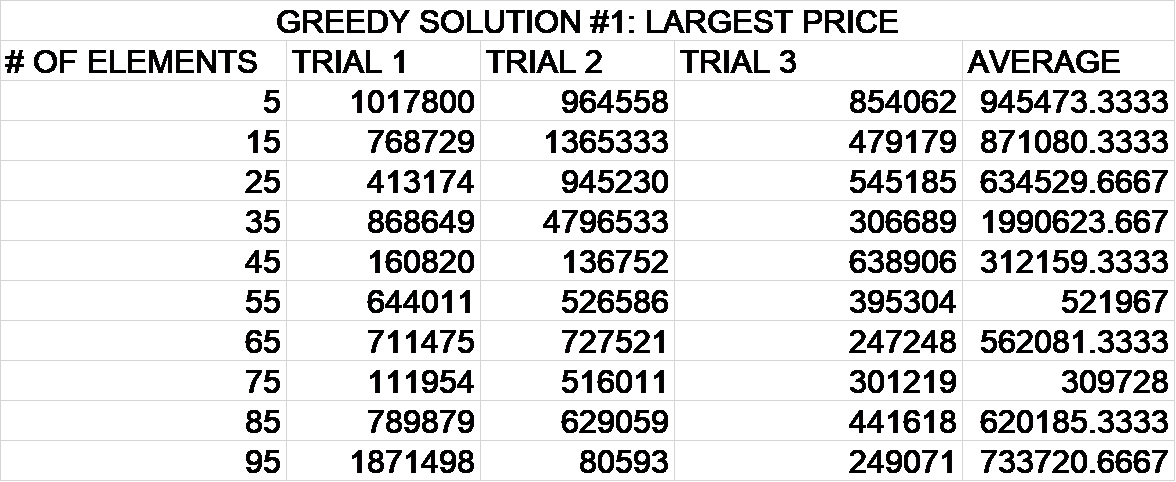
\includegraphics[width=0.8\linewidth]{./largestPriceTable.png}
\caption{Results from Greedy 1: Largest Price Solution}
\label{fig:largestPriceResults}
\end{figure}

\begin{figure}[H]
\centering
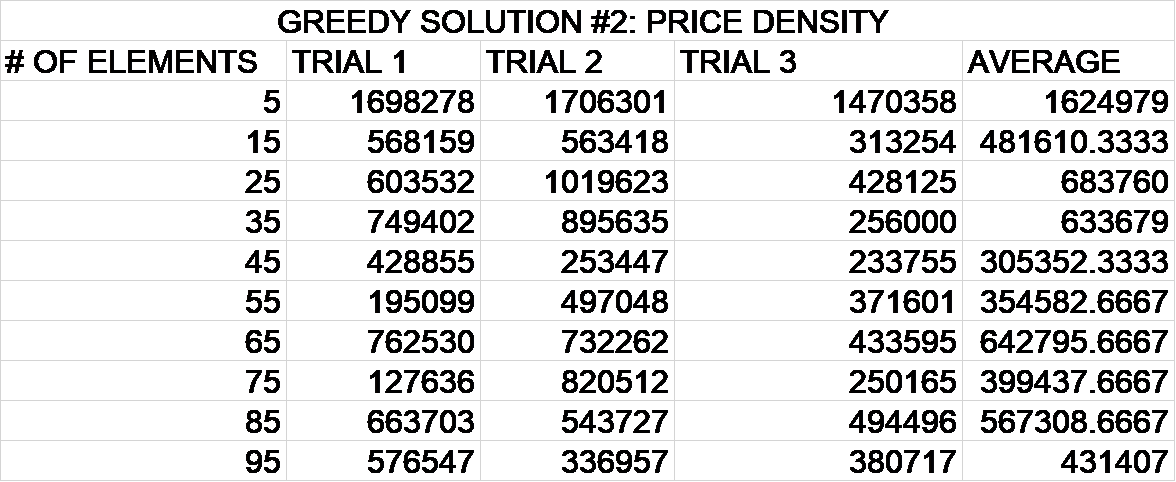
\includegraphics[width=0.8\linewidth]{./priceDensityTable.png}
\caption{Results from Greedy 2: Price Density Solution}
\label{fig:priceDensityResults}
\end{figure}



\subsection{Problems Encountered}
An issue that was encountered with this experiment was with the use of Sahni's algorithm for the dynamic programming solution. He refers to his arrays as being 1-relative, so, it caused errors when his code was copied exactly as it was in the PDF scan provided. In addition, Sahni's code will not work if the first item checked has a weight larger than the capacity. Finally, it seems that Sahni's code does not always return the optimal value when compared to that of brute force. This can be seen because the results yielded by Sahni's code often take up a smaller capacity than that of brute force.

\section{Experimental Analysis}

When comparing these four strategies, the dynamic programming method seems to be the fastest with a total average time of 534512 nanoseconds. The second fastest seems to be Greedy 2 with a total average time of about 612491 nanoseconds. The third fastest seems to be Greedy 1 with a total average time of about 750154 nanoseconds. Finally, the slowest solution method is the brute force with a total average time of 616281688 nanoseconds. While the dynamic programming method was the fastest, it did not seem to return the optimal solution as given by the brute force method. I believe that the results for the dynamic programming solution may be off because, based on further reading and research, it should yield the optimal solution. The graph for the dynamic programming average times, shown in Figure~\ref{fig:dpGraph} shows the total time decreasing as the capacity increases. This may be because, with this type of solution, values do not have to be recalculated, as they do in brute force. Instead, they are saved in a 2-dimensional array which represents a table of values and can be referred to when other values are being calculated. According to Cormen in \textit{Introduction to Algorithms}, the price density algorithm should take $O(nlgn)$ time to run, as seen in the graph in Figure~\ref{fig:Onlgn}. The dynamic programming method should take about $O(nm)$ where $m$ is the number of items in the array of possible items. In this case, $m = 10$ and $O(n*10)$ can be simplified to $O(n)$ as seen in the graph in Figure ~\ref{fig:On}. In the brute force solution, the for loop runs approximately $2^n$ times, giving it a larger time complexity than any of the other solutions, as shown by the fewer results able to be calculated from that solution. 

\begin{figure}[H]
\centering
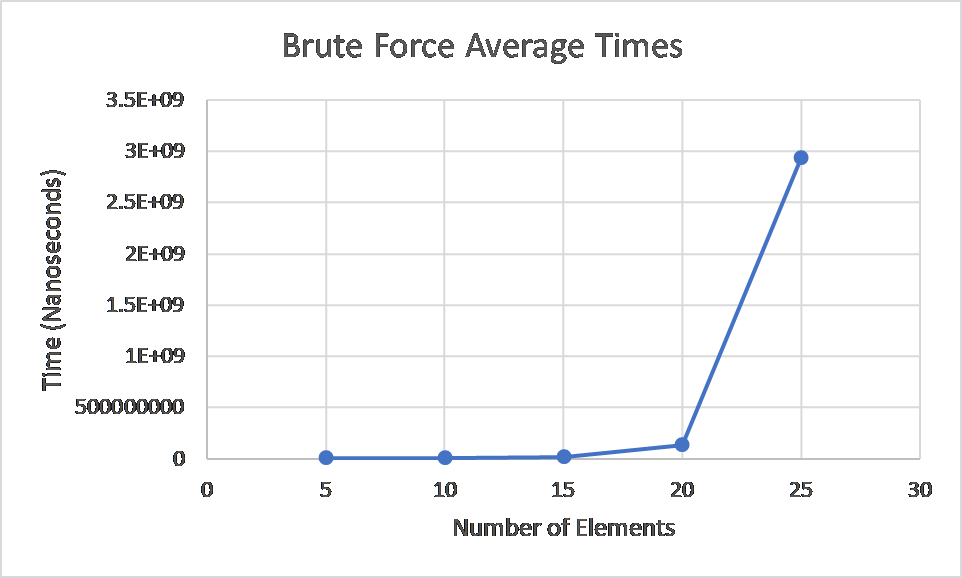
\includegraphics[width=0.8\linewidth]{./bruteForce.png}
\caption{Graph for Brute Force Solution}
\label{fig:bruteForceGraph}
\end{figure}

\begin{figure}[H]
\centering
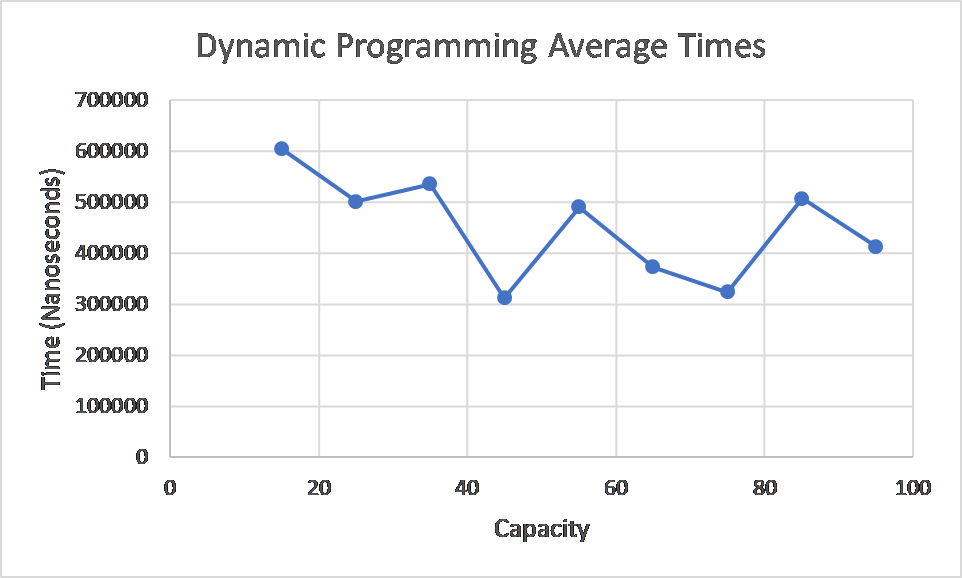
\includegraphics[width=0.8\linewidth]{./dynamicProgramming.png}
\caption{Graph for  Dynamic Programming Solution}
\label{fig:dpGraph}
\end{figure}

\begin{figure}[H]
\centering
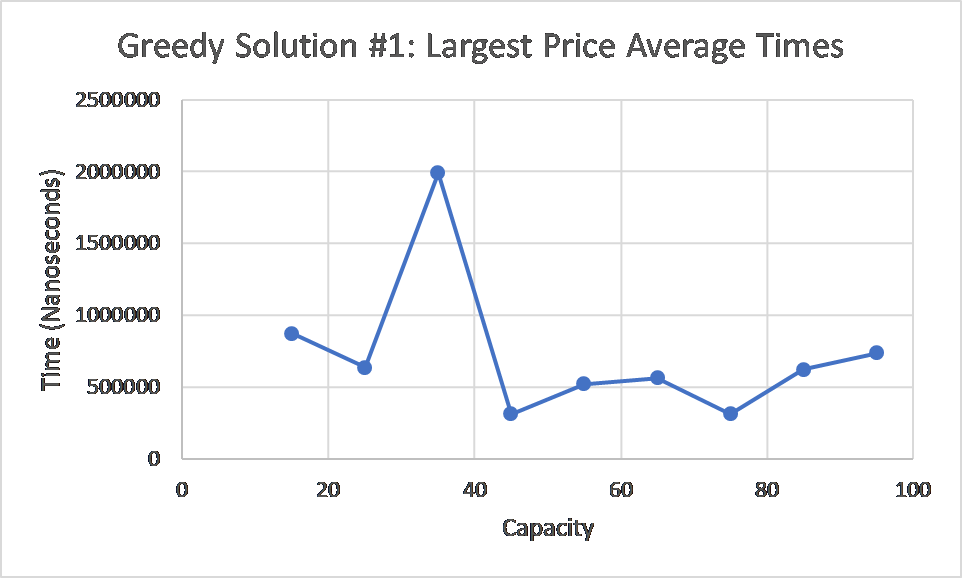
\includegraphics[width=0.8\linewidth]{./largestPrice.png}
\caption{Graph for Greedy 1: Largest Price Solution}
\label{fig:largestPriceGraph}
\end{figure}

\begin{figure}[H]
\centering
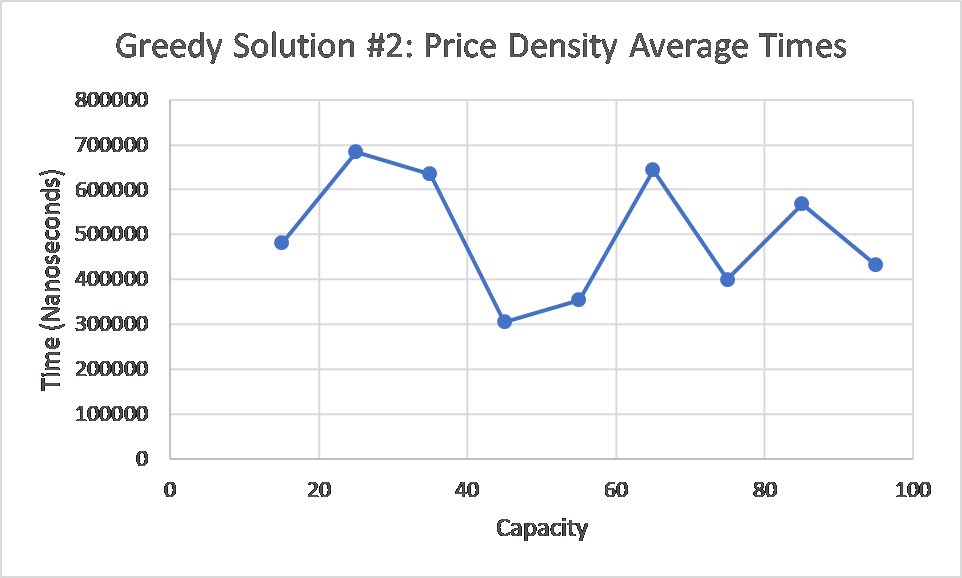
\includegraphics[width=0.8\linewidth]{./priceDensity.png}
\caption{Graph for  Greedy 2: Price Density Solution}
\label{fig:priceDensityGraph}
\end{figure}

\begin{figure}[H]
\centering
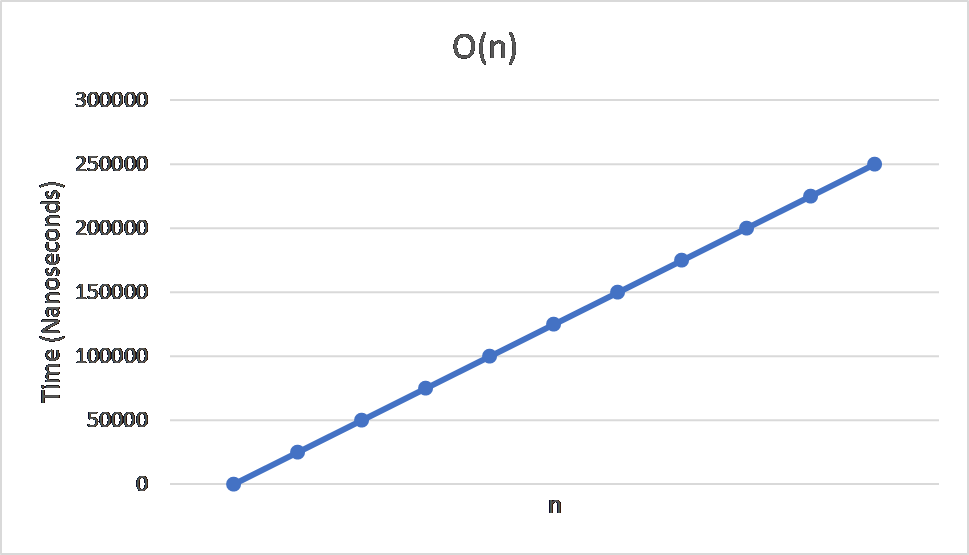
\includegraphics[width=0.8\linewidth]{./On.png}
\caption{Graph of $O(n)$}
\label{fig:On}
\end{figure}

\begin{figure}[H]
\centering
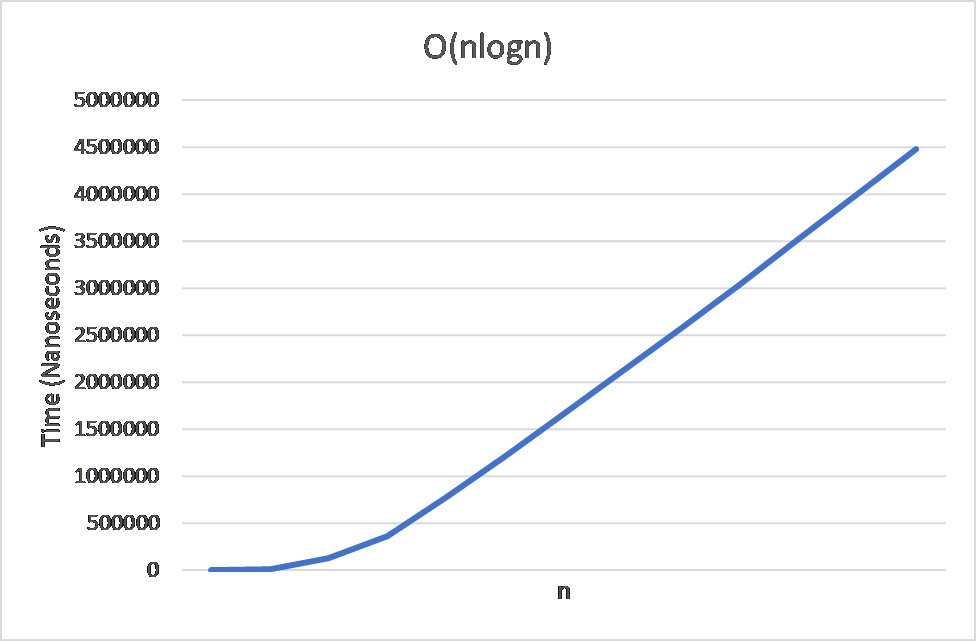
\includegraphics[width=0.8\linewidth]{./Onlgn.png}
\caption{Graph of $O(nlogn)$}
\label{fig:Onlgn}
\end{figure}

\section{Conclusions}
If the knapsack capacity is smaller, it may be feasible to use the brute force solution, but, as the capacity grows larger, so does the time it takes for this solution to finish. The best solution time-wise and accuracy-wise is the dynamic programming solution because, even though, from these results, it does not always provide the optimal solution, the total time appears to decrease as the capacity of the knapsack increases and the solutions seem to be most similar to those of the brute force method. Another testing method that may be helpful in order to yield more results is keeping the capacity constant and changing the number of possible items to see how long it takes to fit more and more items into a specific capacity with each solution method. It is also important to consider the positive aspects of greedy algorithms and the fact that they are more likely to be used in real-world situations, in which a ``good enough" solution could be acceptable, than the more tedious solutions, like brute force and dynamic programming, which would give more exact solutions.



\begin{thebibliography}{}


\bibitem{cormen2001introduction}
T.~H. Cormen, C.~E. Leiserson, R.~L. Rivest, C.~Stein.,
\emph{{Introduction to Algorithms, 3rd Edition}}.
MIT press Cambridge, 2001.

\end{thebibliography}


\newpage
\section*{Appendix A}
\normalsize{JAVA Source Code:  \textbf{BruteForce.java}}
\footnotesize{
	\lstinputlisting{BruteForce.java}}
\normalsize{JAVA Source Code:  \textbf{DP2.java}}
\footnotesize{
	\lstinputlisting{DP2.java}}
\normalsize{JAVA Source Code:  \textbf{GreedyDensity.java}}
\footnotesize{
	\lstinputlisting{GreedyDensity.java}}
\normalsize{JAVA Source Code:  \textbf{GreedyPrice.java}}
\footnotesize{
	\lstinputlisting{GreedyPrice.java}}
\normalsize{JAVA Source Code:  \textbf{Item.java}}
\footnotesize{
	\lstinputlisting{Item.java}}
\normalsize{JAVA Source Code:  \textbf{Knapsack.java}}
\footnotesize{
	\lstinputlisting{Knapsack.java}}
\normalsize{JAVA Source Code:  \textbf{Simulation.java}}
\footnotesize{
	\lstinputlisting{Simulation.java}}
\normalsize{JAVA Source Code:  \textbf{Sort.java}}
\footnotesize{
	\lstinputlisting{Sort.java}}


\end{document}